\section{Choice of Hyperparameters}

This section will discuss and try to validate the choice of all the
hyperparameters necessary for the training of a \acrshort{gp} model to capture
the CARNOT building's behaviour.

As described in Section~\ref{sec:gp_dynamical_system}, for the purpose of this
project the \acrlong{gp} model will be trained using the \acrshort{narx}
structure.

\subsection{Lengthscales}

\subsection{The Kernel}

\subsection{Loss functions}

The most important metric for measuring the performance of a model is the value
of the loss function, computed on a dataset separate from the one used for
training.

There exist a number of different loss functions, each focusing on different
aspects of a model's performance. A selection of loss functions used in
identification of Gaussian Process models is presented
below~\cite{kocijanModellingControlDynamic2016}.

The \acrfull{rmse} is a very commonly used performance measure. As the name
suggests, it computes the root of the mean squared error:

\begin{equation}\label{eq:rmse}
    \text{RMSE} = \sqrt{\frac{1}{N}\sum_{i=1}^N \left(y_i -
    E(\hat{y}_i)\right)^{2}}
\end{equation}

This performance metric is very useful when training a model whose goal is
solely to minimize the difference between the values measured, and the ones
predicted by the model.

A variant of the \acrshort{mse} is the \acrfull{smse}, which normalizes the
\acrlong{mse} by the variance of the output values of the validation dataset.

\begin{equation}\label{eq:smse}
    \text{SMSE} = \frac{1}{N}\frac{\sum_{i=1}^N \left(y_i -
    E(\hat{y}_i)\right)^{2}}{\sigma_y^2}
\end{equation}

While the \acrshort{rmse} and the \acrshort{smse} are very good at ensuring the
predicted mean value of the Gaussian Process is close to the measured values of
the validation dataset, the confidence of the Gaussian Process prediction is
completely ignored. In this case two models predicting the same mean values, but
having very differnt confidence intervals would be equivalent according to these
performance metrics.

The \acrfull{lpd} is a performance metric which takes into account not only the
the mean value of the GP prediction, but the entire distribution:

\begin{equation}
    \text{LPD} = \frac{1}{2} \ln{\left(2\pi\right)} + \frac{1}{2N}
    \sum_{i=1}^N\left(\ln{\left(\sigma_i^2\right)} + \frac{\left(y_i -
    E(\hat{y}_i)\right)^{2}}{\sigma_i^2}\right)
\end{equation}

where $\sigma_i^2$ is the model's output variance at the \textit{i}-th step.
The \acrshort{lpd} scales the error of the mean value prediction $\left(y_i -
E(\hat{y}_i)\right)^{2}$ by the variance $\sigma_i^2$. This means that the
overconfident models get penalized more than the more conservative models for
the same mean prediction error, leading to models that better represent
the real system. 

The \acrfull{msll} is obtained by substacting the loss of the model that
predicts using a Gaussian with the mean $E(\boldsymbol{y})$ and variance
$\sigma_y^2$ of the measured data from the model \acrshort{lpd} and taking the
mean of the obtained result:

\begin{equation}
    \text{MSLL} = \frac{1}{2N}\sum_{i=1}^N\left[
        \ln{\left(\sigma_i^2\right) + \frac{\left(y_i -
        E\left(\hat{y}_i\right)\right)^2}{\sigma_i^2}}
    \right] - \frac{1}{2N}\sum_{i=1}^N\left[
        \ln{\left(\sigma_y^2\right) + \frac{\left(y_i -
        E\left(\boldsymbol{y}\right)\right)^2}{\sigma_y^2}}
    \right]
\end{equation}

The \acrshort{msll} is approximately zero for simple models and negative for
better ones.

% TODO: [Hyperparameters] Explain loss table, difference in lags, etc.
\begin{table}[ht]
%\vspace{-8pt}
\centering
    \begin{tabular}{||c c c|c c c c||}
        \hline
        \multicolumn{3}{||c|}{Lags} & \multicolumn{4}{c||}{Loss functions}\\
        w & u & y & RMSE & SMSE & MSLL & LPD\\
        \hline \hline
        1 & 1 & 1 & 0.3464 & 0.36394 & 20.74 & 21.70 \\
        1 & 1 & 2 & 0.1415 & 0.06179 & -9.62 & -8.67 \\
        1 & 1 & 3 & 0.0588 & 0.01066 & -8.99 & -8.03 \\
        1 & 2 & 1 & 0.0076 & 0.00017 & 71.83 & 72.79 \\
        1 & 2 & 3 & \textbf{0.0041} & \textbf{0.00005} & 31.25 & 32.21 \\
        2 & 1 & 2 & 0.1445 & 0.06682 & -9.57 & -8.61 \\
        2 & 1 & 3 & 0.0797 & 0.02033 & -10.94 & -9.99 \\
        3 & 1 & 3 & 0.0830 & 0.02219 & \textbf{-11.48} & \textbf{-10.53} \\
        3 & 2 & 2 & 0.0079 & 0.00019 & 58.30 & 59.26 \\
        \hline
    \end{tabular}
\caption{GP Loss function values for different autoregressive lags}
\label{tab:GP_loss_functions}
\end{table}


\begin{table}[ht]
%\vspace{-8pt}
\centering
    \resizebox{\columnwidth}{!}{%
    \begin{tabular}{||c c c|c|c c c c c c c c c c c||}
        \hline
        \multicolumn{3}{||c|}{Lags} & Variance &\multicolumn{11}{c||}{Kernel
        lengthscales relative importance} \\
            w & u & y & $\sigma^2$ &$\lambda_{w1,1}$ & $\lambda_{w1,2}$ &
            $\lambda_{w1,3}$ & $\lambda_{w2,1}$ & $\lambda_{w2,2}$ &
            $\lambda_{w2,3}$ & $\lambda_{u1,1}$ & $\lambda_{u1,2}$ &
            $\lambda_{y1,1}$ & $\lambda_{y1,2}$ & $\lambda_{y1,3}$\\
        \hline \hline
        1 & 1 & 1 & 0.11 & 0.721 &  &  & 2.633 &  &  & 0.569 &  & 2.645 &  &  \\
        1 & 1 & 2 & 22.68 & 0.222 &  &  & 0.751 &  &  & 0.134 &  & 3.154 & 3.073
          &  \\ 1 & 1 & 3 & 0.29 & 0.294 &  &  & 1.303 &  &  & 0.356 &  & 2.352
          & 1.361 & 2.045 \\ 1 & 2 & 1 & 7.55 & 0.157 &  &  & 0.779 &  &  &
        0.180 & 0.188 & 0.538 &  &  \\ 1 & 2 & 3 & 22925.40 & 0.018 &  &  &
        0.053 &  &  & 0.080 & 0.393 & 0.665 & 0.668 & 0.018 \\ 2 & 1 & 2 & 31.53
              & 0.010 & 0.219 &  & 0.070 & 0.719 &  & 0.123 &  & 3.125 & 3.044 &
              \\ 2 & 1 & 3 & 0.44 & 0.007 & 0.251 &  & 0.279 & 1.229 &  & 0.319
                   &  & 2.705 & 1.120 & 2.510 \\ 3 & 1 & 3 & 0.56 & 0.046 &
              0.064 & 0.243 & 0.288 & 1.151 & 0.233 & 0.302 &  & 2.809 & 1.086 &
              2.689 \\ 3 & 2 & 2 & 1.65 & 0.512 & 0.074 & 0.201 & 0.161 & 1.225
                         & 0.141 & 0.231 & 0.331 & 0.684 & 0.064 &  \\
        \hline
    \end{tabular}%
    }
\caption{GP hyperparameter values for different autoregressive lags}
\label{tab:GP_hyperparameters}
\end{table}


\begin{table}[ht]
%\vspace{-8pt}
\centering
    \begin{tabular}{||c c c|c c c c||}
        \hline
        \multicolumn{3}{||c|}{Lags} & \multicolumn{4}{c||}{Loss functions}\\
        w & u & y & RMSE & SMSE & MSLL & LPD\\
        \hline \hline
        1 & 1 & 1 & 0.3253 & 0.3203 & 228.0278 & 228.9843 \\
        1 & 1 & 2 & 0.2507 & 0.1903 & 175.5525 & 176.5075 \\
        1 & 1 & 3 & 0.1983 & 0.1192 & 99.7735 & 100.7268 \\
        1 & 2 & 1 & 0.0187 & 0.0012 & -9.5386 & -8.5836 \\
        1 & 2 & 3 & \textbf{0.0182} & \textbf{0.0011} & \textbf{-10.2739} &
        \textbf{-9.3206} \\
        2 & 1 & 2 & 0.2493 & 0.1884 & 165.0734 & 166.0284 \\
        2 & 1 & 3 & 0.1989 & 0.1200 & 103.6753 & 104.6287 \\
        3 & 1 & 3 & 0.2001 & 0.1214 & 104.4147 & 105.3681 \\
        3 & 2 & 2 & 0.0206 & 0.0014 & -9.9360 & -8.9826 \\
        \hline
    \end{tabular}
\caption{SVGP Loss function values for different autoregressive lags}
\label{tab:SVGP_loss_functions}
\end{table}

\begin{table}[ht]
%\vspace{-8pt}
\centering
    \resizebox{\columnwidth}{!}{%
    \begin{tabular}{||c c c|c|c c c c c c c c c c c||}
        \hline
        \multicolumn{3}{||c|}{Lags} & Variance &\multicolumn{11}{c||}{Kernel
        lengthscales relative importance} \\
            w & u & y & $\sigma^2$ &$\lambda_{w1,1}$ & $\lambda_{w1,2}$ &
            $\lambda_{w1,3}$ & $\lambda_{w2,1}$ & $\lambda_{w2,2}$ &
            $\lambda_{w2,3}$ & $\lambda_{u1,1}$ & $\lambda_{u1,2}$ &
            $\lambda_{y1,1}$ & $\lambda_{y1,2}$ & $\lambda_{y1,3}$\\
        \hline \hline
                1 & 1 & 1 & 0.2970 & 0.415 &  &  & 0.748 &  &  & 0.675 &  & 0.680 &  &  \\
        1 & 1 & 2 & 0.2717 & 0.430 &  &  & 0.640 &  &  & 0.687 &  & 0.559 & 0.584 &  \\
        1 & 1 & 3 & 0.2454 & 0.455 &  &  & 0.589 &  &  & 0.671 &  & 0.522 & 0.512 & 0.529 \\
        1 & 2 & 1 & 0.2593 & 0.310 &  &  & 0.344 &  &  & 0.534 & 0.509 & 0.597 &  &  \\
        1 & 2 & 3 & 0.2139 & 0.330 &  &  & 0.368 &  &  & 0.537 & 0.447 & 0.563 & 0.410 & 0.363 \\
        2 & 1 & 2 & 0.2108 & 0.421 & 0.414 &  & 0.519 & 0.559 &  & 0.680 &  & 0.525 & 0.568 &  \\
        2 & 1 & 3 & 0.1795 & 0.456 & 0.390 &  & 0.503 & 0.519 &  & 0.666 &  & 0.508 & 0.496 & 0.516 \\
        3 & 1 & 3 & 0.1322 & 0.432 & 0.370 & 0.389 & 0.463 & 0.484 & 0.491 & 0.666 &  & 0.511 & 0.501 & 0.526 \\
        3 & 2 & 2 & 0.1228 & 0.329 & 0.317 & 0.325 & 0.334 & 0.337 & 0.331 &
        0.527 & 0.441 & 0.579 & 0.435 &  \\
        \hline
    \end{tabular}%
    }
\caption{SVGP hyperparameter values for different autoregressive lags}
\label{tab:SVGP_hyperparameters}
\end{table}

\clearpage

\subsection{Validation of hyperparameters}

% TODO: [Hyperparameters] Validation of hyperparameters

\subsubsection{Conventional Gaussian Process}

\begin{figure}[ht]
    \centering
    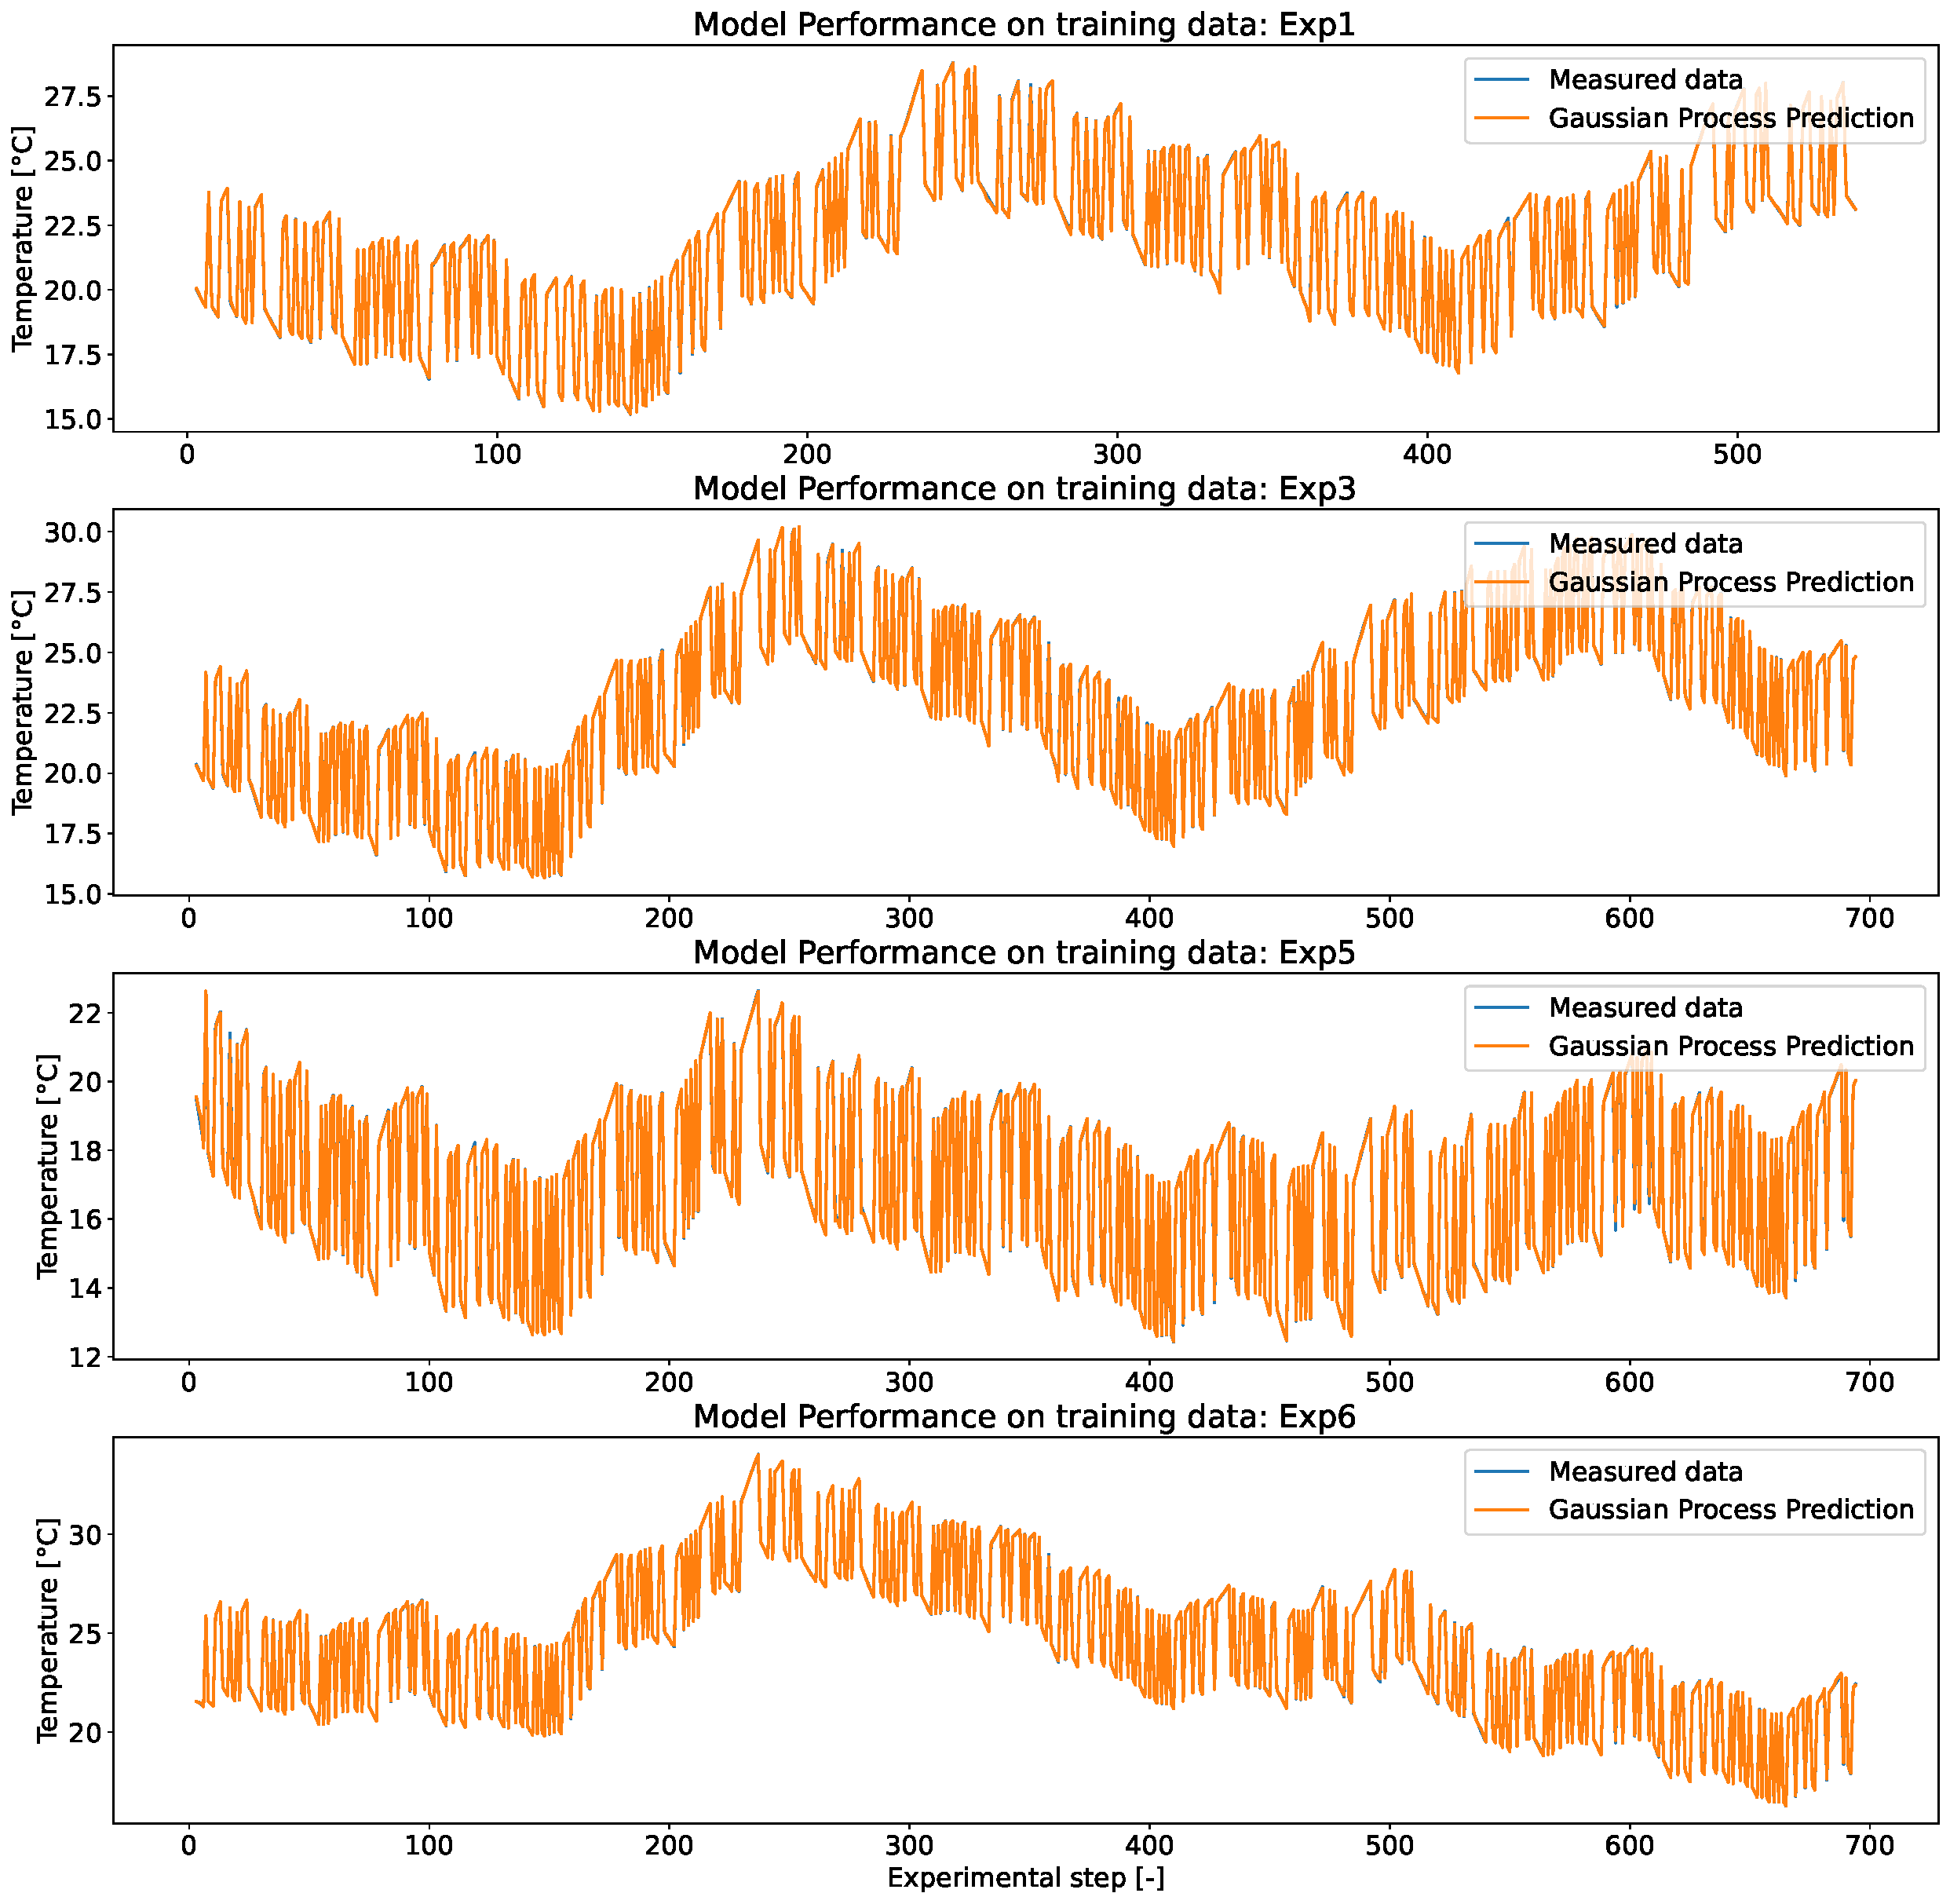
\includegraphics[width = \textwidth]{Plots/GP_113_training_performance.pdf}
    \caption{}
    \label{fig:GP_train_validation}
\end{figure}

\begin{figure}[ht]
    \centering
    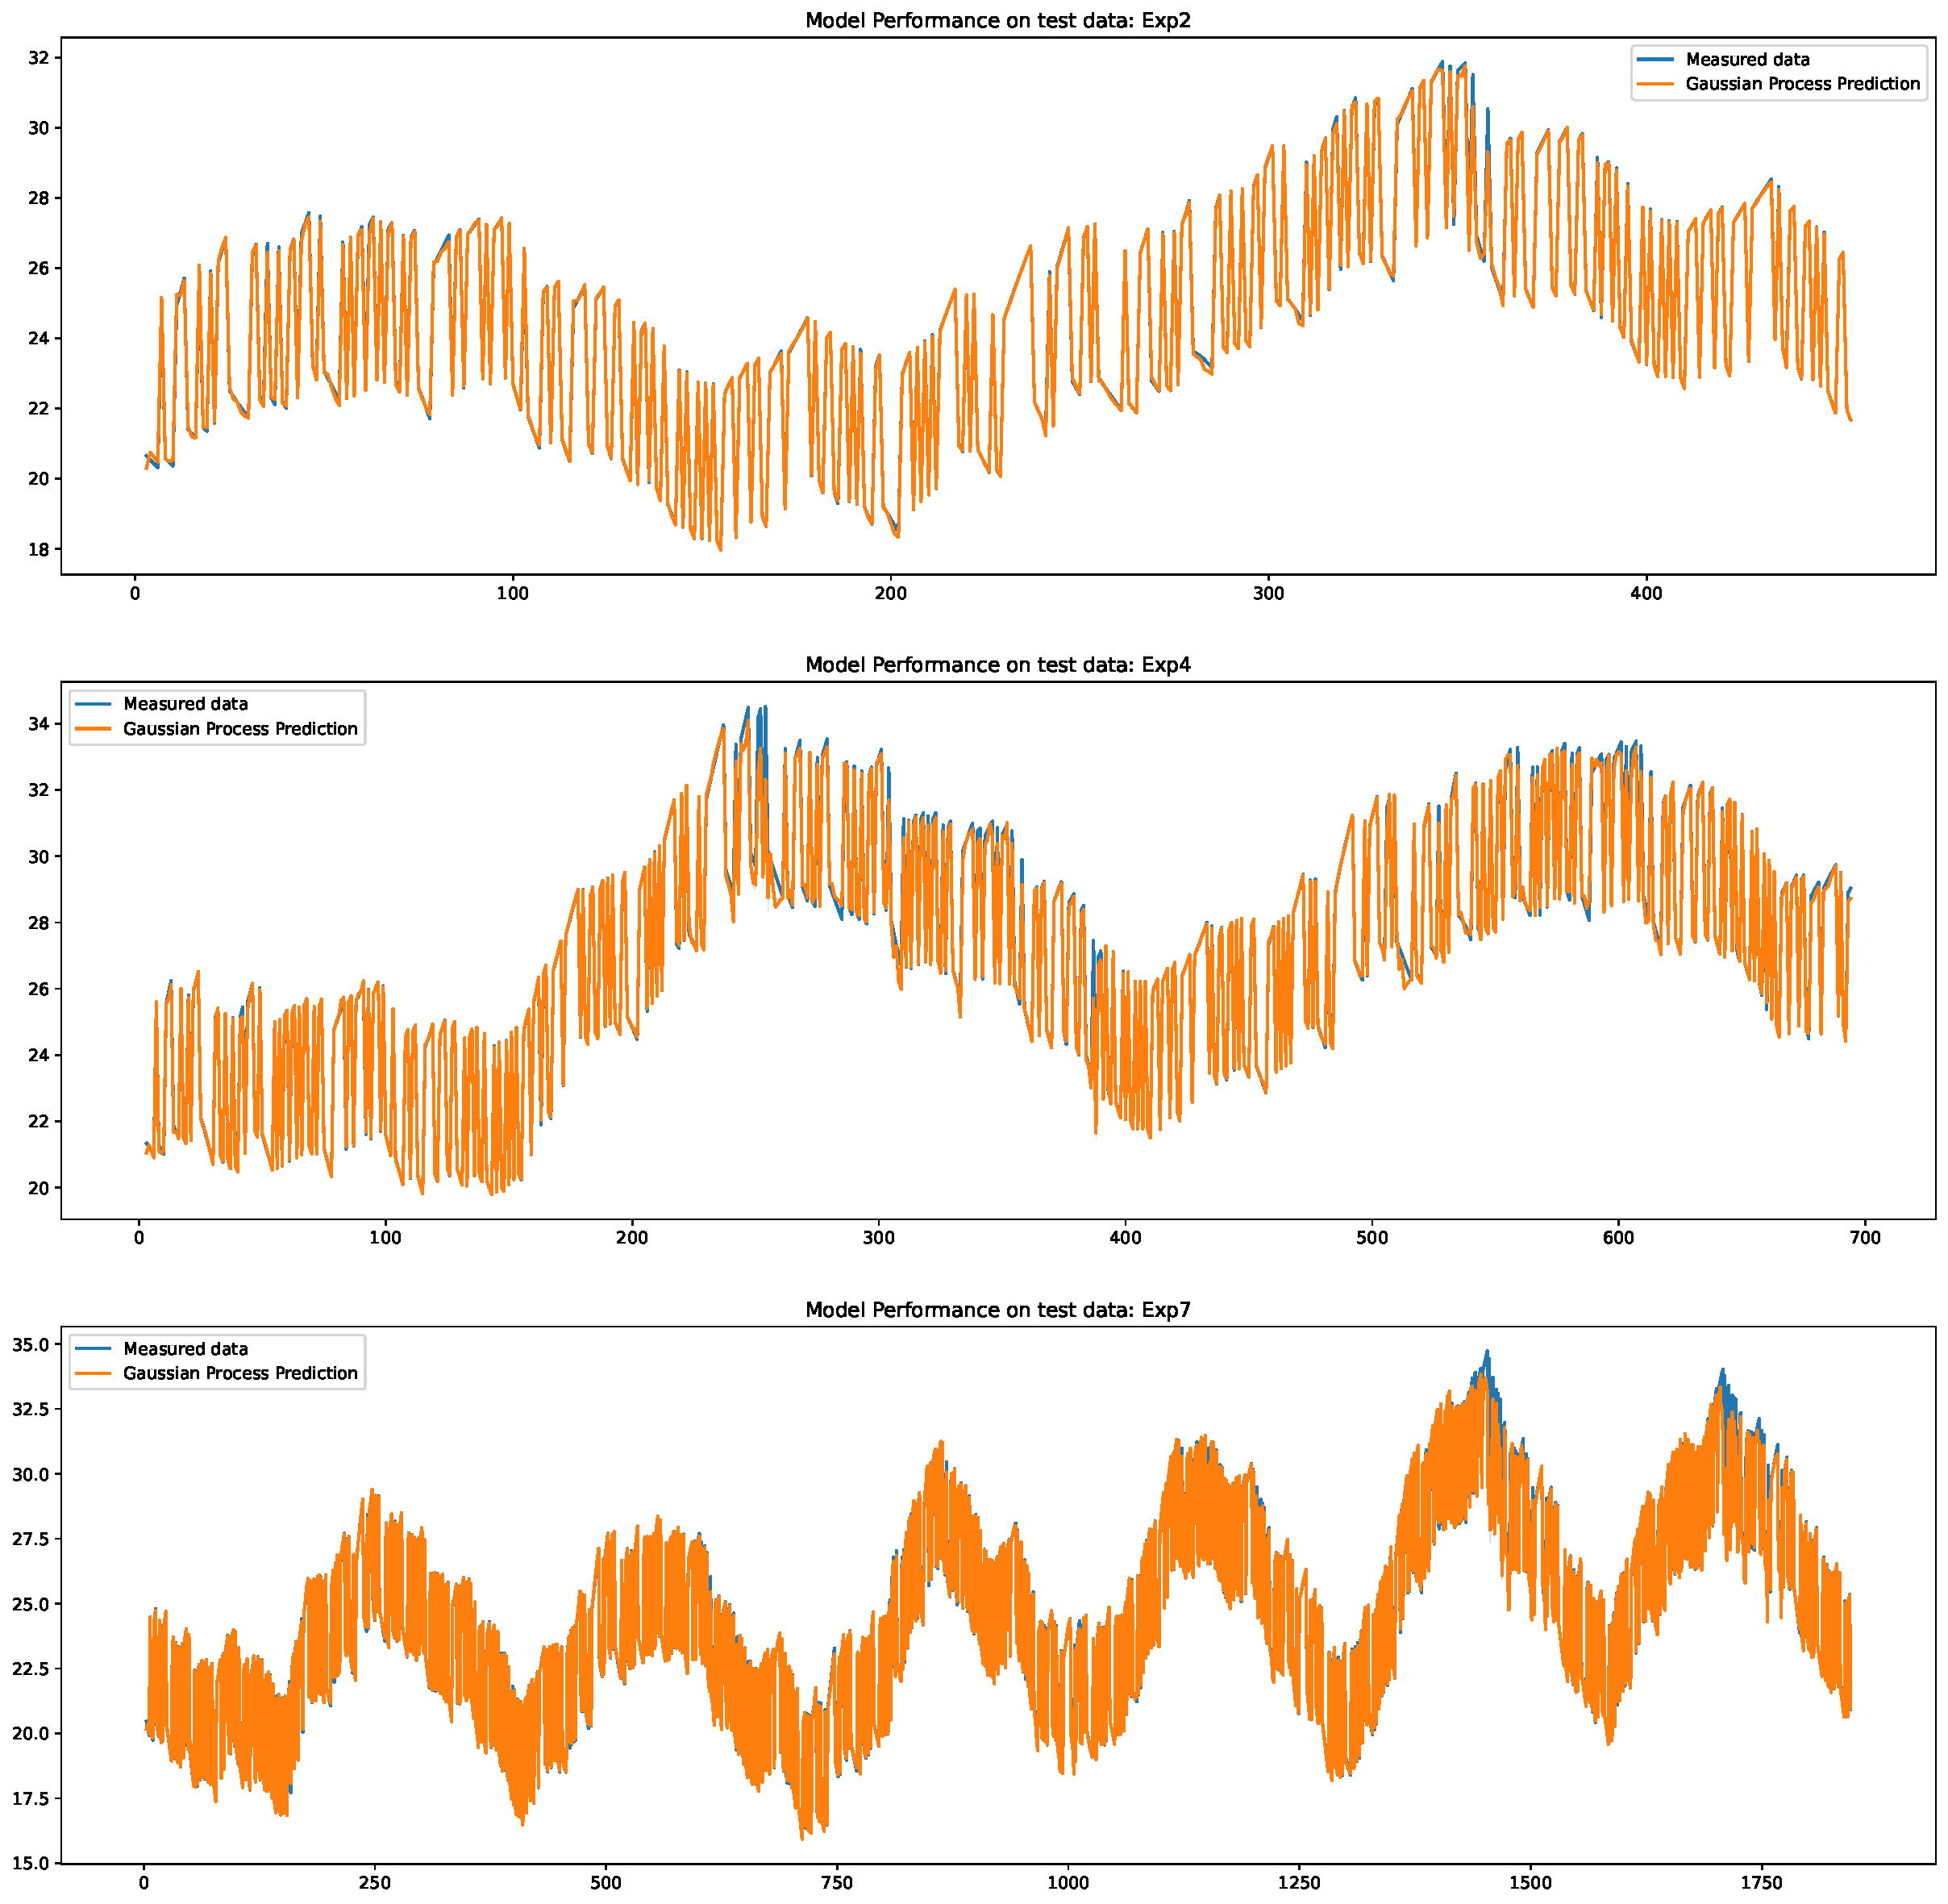
\includegraphics[width = \textwidth]{Plots/GP_113_test_performance.pdf}
    \caption{}
    \label{fig:GP_test_validation}
\end{figure}


\begin{figure}[ht]
    \centering
    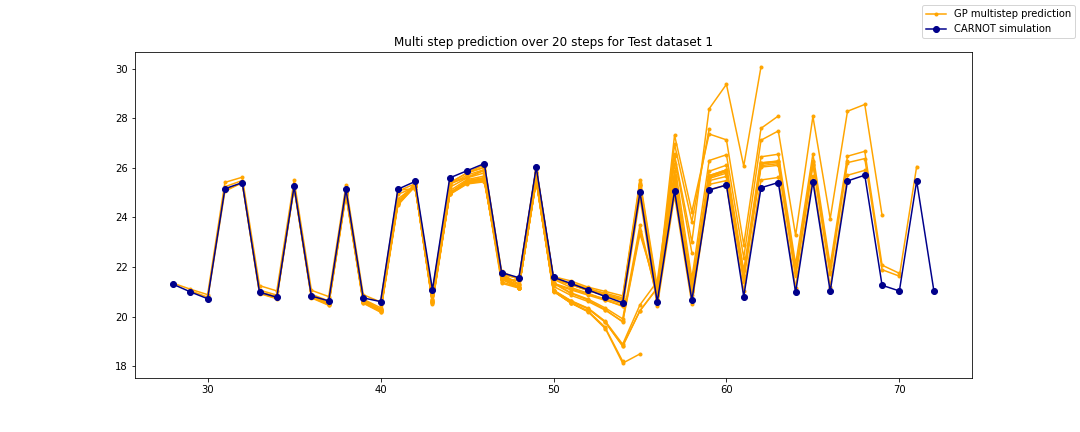
\includegraphics[width =
    \textwidth]{Plots/GP_113_-1pts_test_prediction_20_steps.png}
    \caption{}
    \label{fig:GP_multistep_validation}
\end{figure}

\clearpage

\subsubsection{Sparse and Variational Gaussian Process}

\begin{figure}[ht]
    \centering
    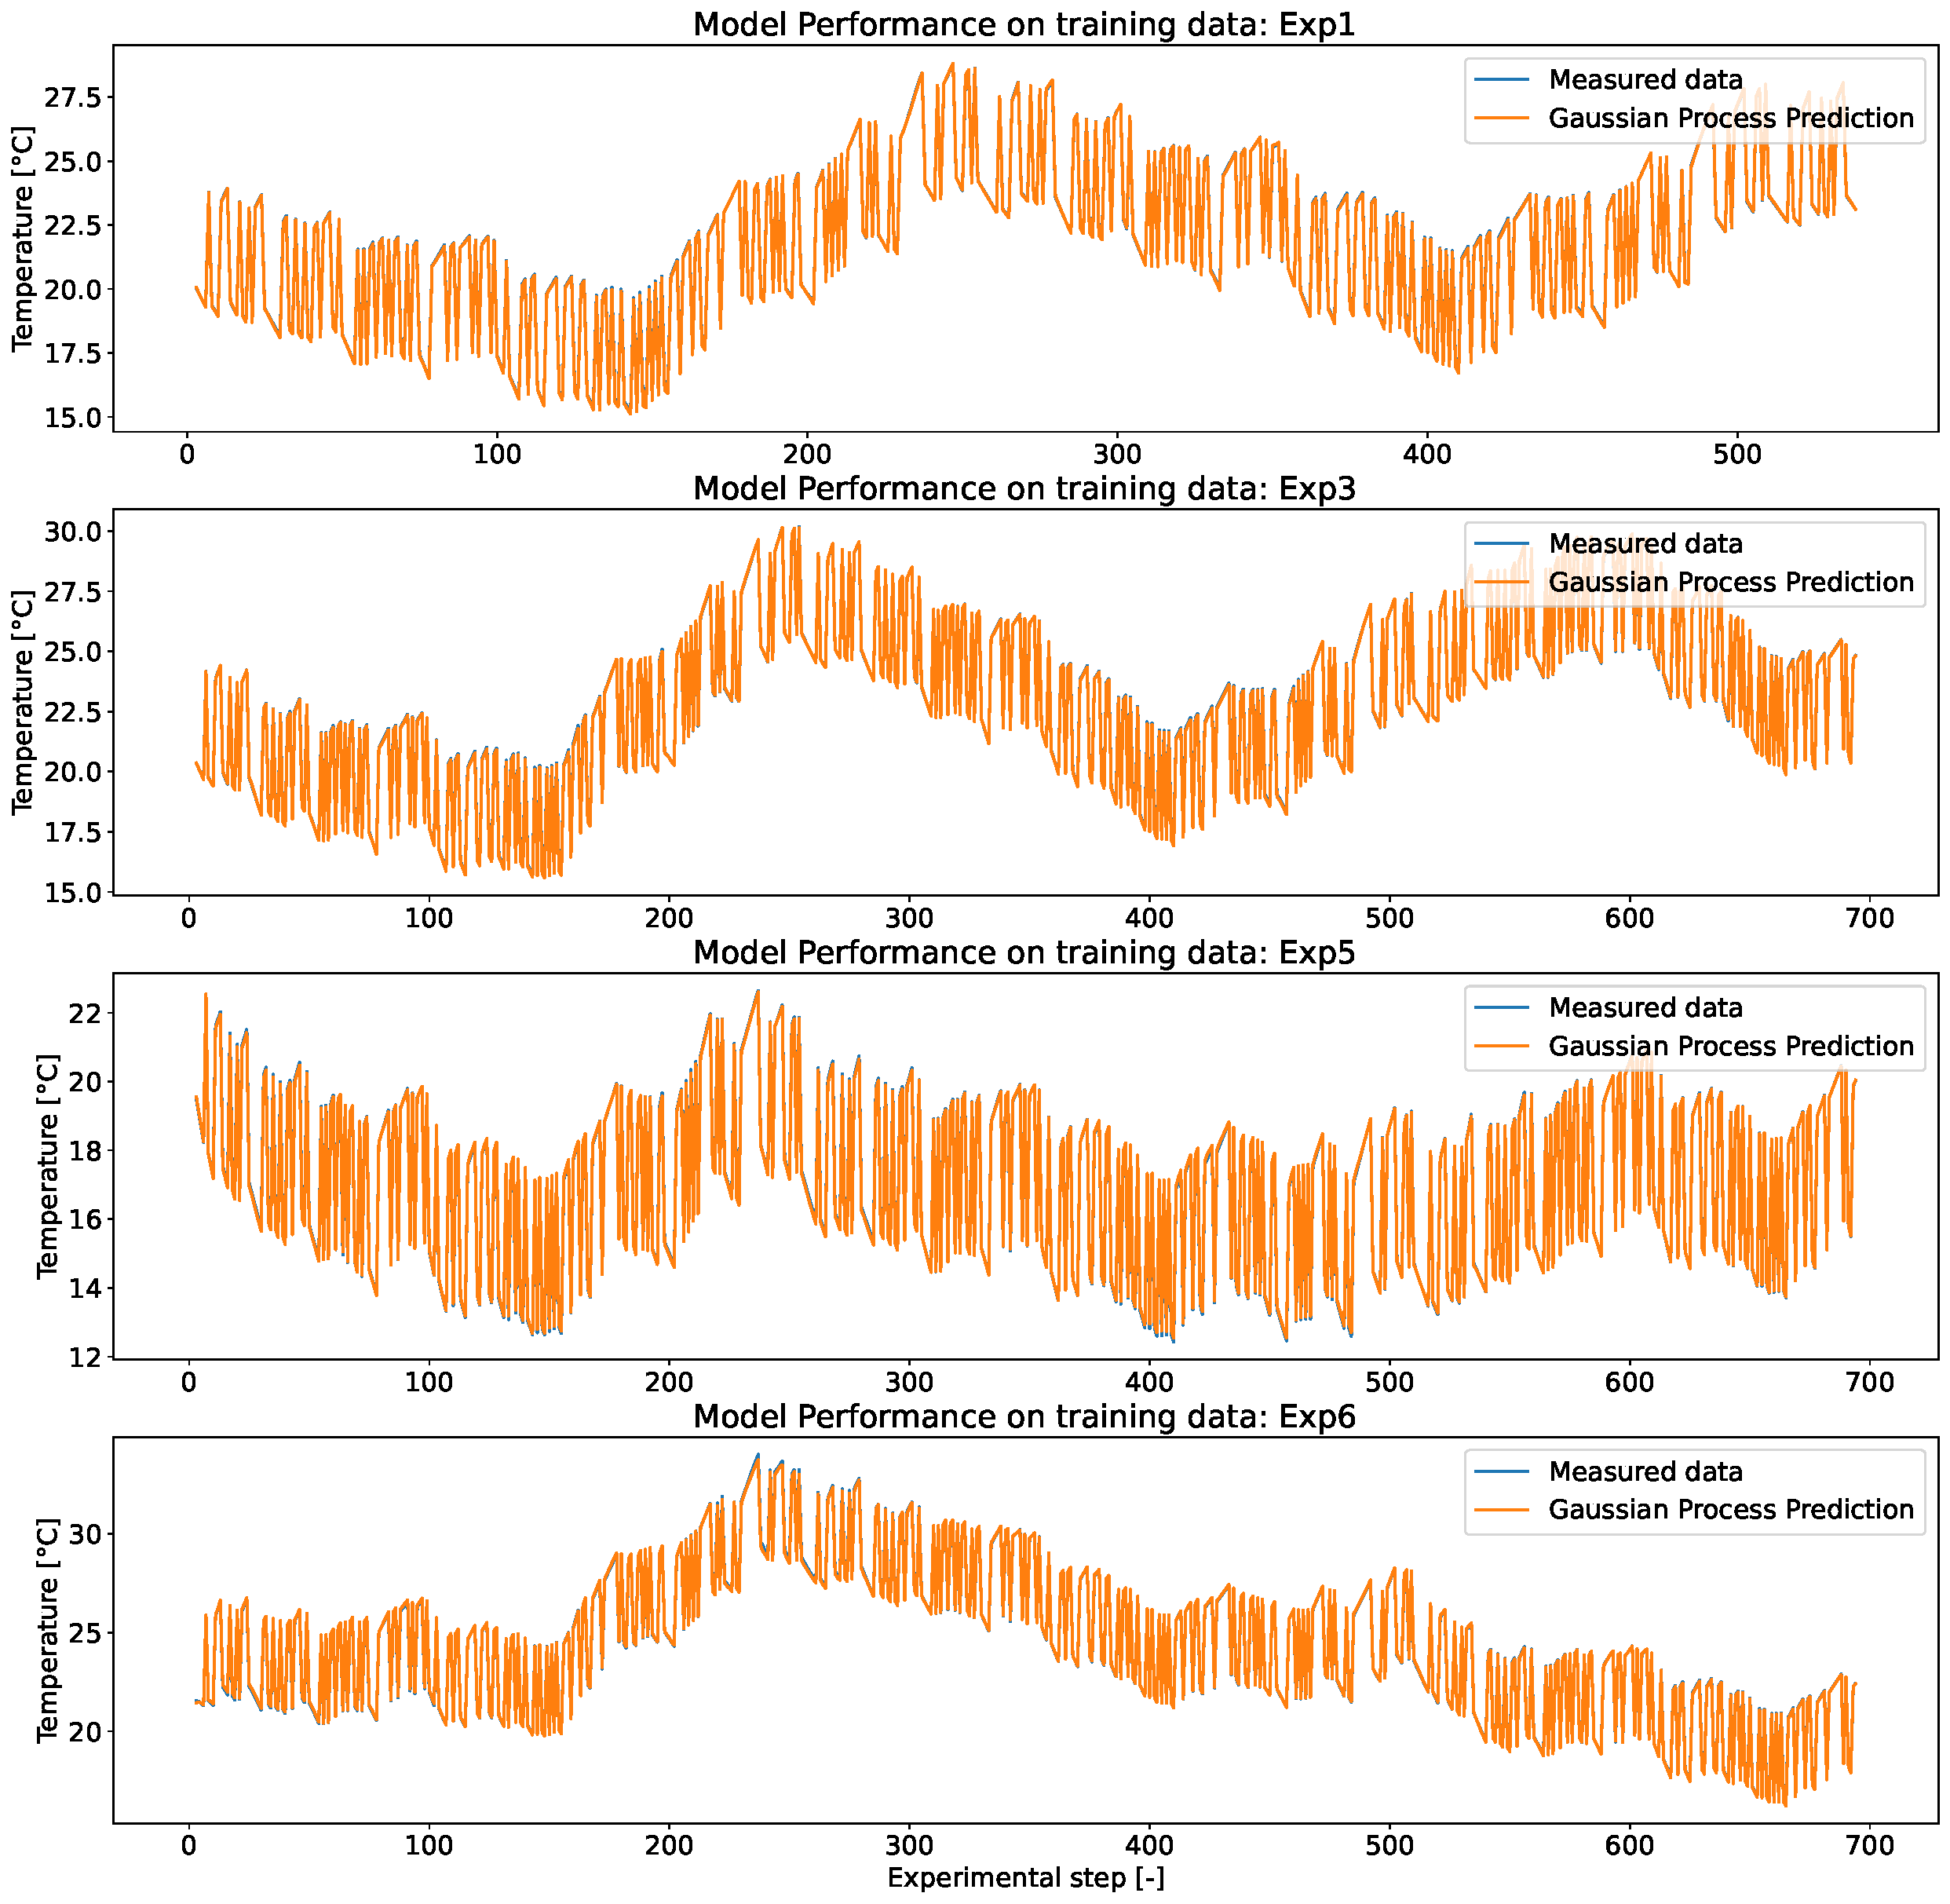
\includegraphics[width = \textwidth]{Plots/SVGP_123_training_performance.pdf}
    \caption{}
    \label{fig:SVGP_train_validation}
\end{figure}

\begin{figure}[ht]
    \centering
    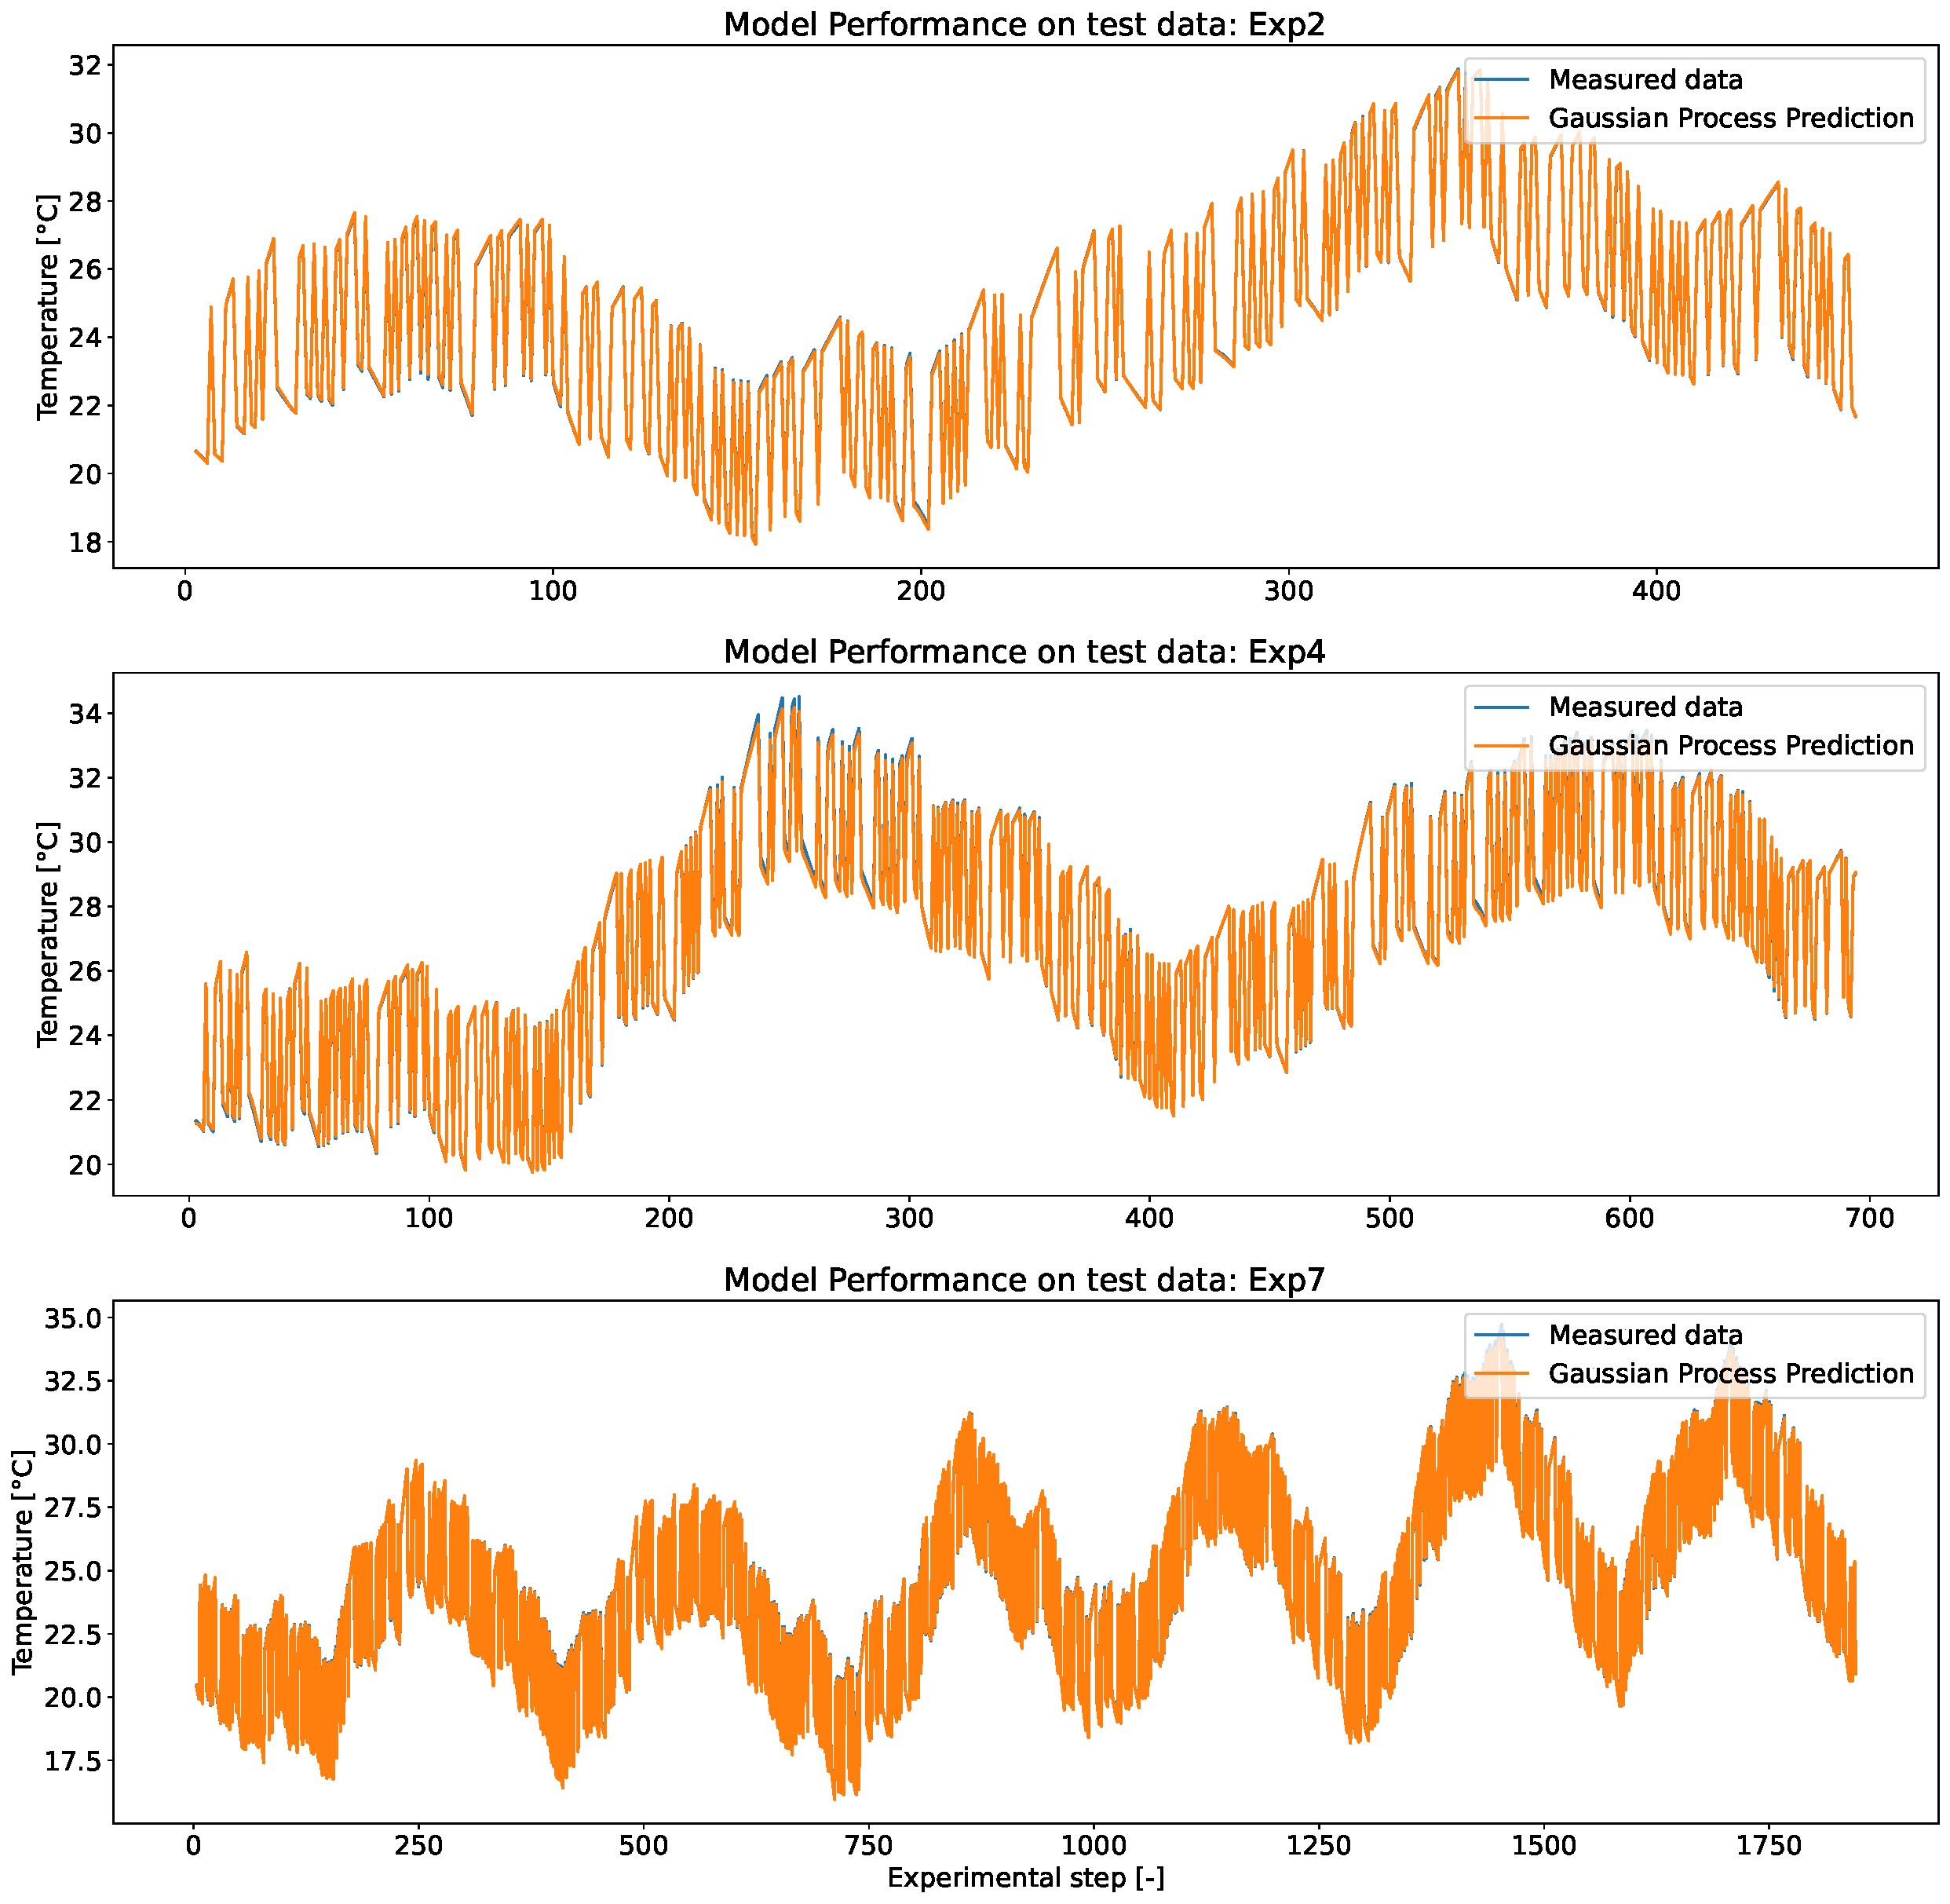
\includegraphics[width = \textwidth]{Plots/SVGP_123_test_performance.pdf}
    \caption{}
    \label{fig:SVGP_test_validation}
\end{figure}

\begin{figure}[ht]
    \centering
    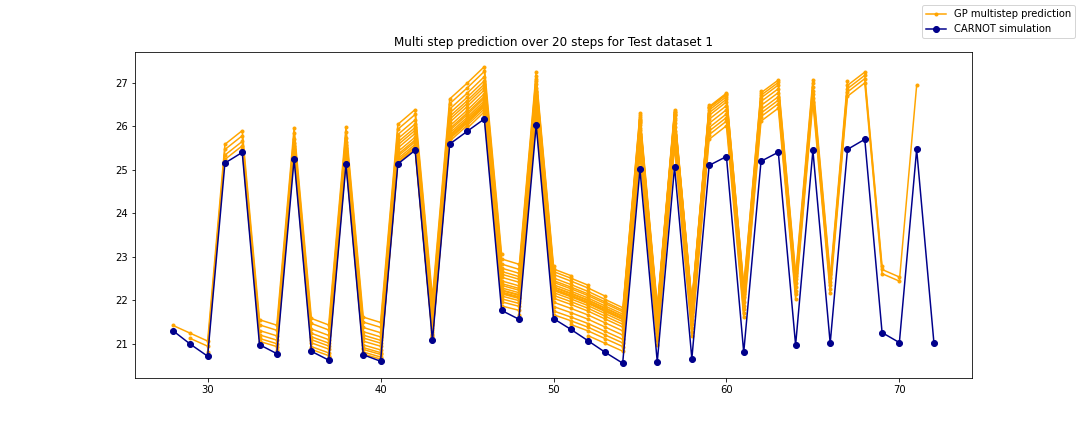
\includegraphics[width =
    \textwidth]{Plots/SVGP_123_test_prediction_20_steps.png}
    \caption{}
    \label{fig:SVGP_multistep_validation}
\end{figure}

\clearpage
